% !TeX document-id = {ee196d1e-6108-43df-9847-6bc01d26e886}
% !TeX TXS-program:pdflatex = pdflatex -synctex=1 -interaction=nonstopmode --shell-escape %.tex
\documentclass[12pt]{report}
\usepackage[utf8]{inputenc}
%\usepackage[14pt]{extsizes}
\usepackage{listings}
\usepackage{indentfirst}
\usepackage{geometry}
\usepackage{textcomp}
\usepackage{amssymb}
\usepackage{amsmath}
\usepackage{amsthm} 
\usepackage{caption}
\usepackage{misccorr}
\usepackage[noadjust]{cite}
\usepackage{cmap} 
\usepackage[T2A]{fontenc}
\usepackage[english, russian]{babel}
\usepackage{graphics}
\usepackage{graphicx}
\usepackage{textcomp}
\usepackage{verbatim}
\usepackage{makeidx}
\usepackage{float}
\usepackage{bm}
\usepackage{esint}
\usepackage{mathtools}
\usepackage{graphicx}
\usepackage{listings}
% Для листинга кода:
\lstset{ %
language=python,                 % выбор языка для подсветки (здесь это С)
basicstyle=\small\sffamily, % размер и начертание шрифта для подсветки кода
numbers=left,               % где поставить нумерацию строк (слева\справа)
numberstyle=\tiny,           % размер шрифта для номеров строк
stepnumber=1,                   % размер шага между двумя номерами строк
numbersep=5pt,                % как далеко отстоят номера строк от подсвечиваемого кода
showspaces=false,            % показывать или нет пробелы специальными отступами
showstringspaces=false,      % показывать или нет пробелы в строках
showtabs=false,             % показывать или нет табуляцию в строках
frame=single,              % рисовать рамку вокруг кода
tabsize=2,                 % размер табуляции по умолчанию равен 2 пробелам
captionpos=t,              % позиция заголовка вверху [t] или внизу [b] 
breaklines=true,           % автоматически переносить строки (да\нет)
breakatwhitespace=false, % переносить строки только если есть пробел
escapeinside={\#*}{*)}  % если нужно добавить комментарии в коде
}


% plot
\usepackage{pgfplots}
\usepackage{filecontents}
\usetikzlibrary{datavisualization}
\usetikzlibrary{datavisualization.formats.functions}

% Для измененных титулов глав:
\usepackage{titlesec, blindtext, color} % подключаем нужные пакеты
\definecolor{gray75}{gray}{0.75} % определяем цвет
\newcommand{\hsp}{\hspace{20pt}} % длина линии в 20pt
% titleformat определяет стиль
\titleformat{\chapter}[hang]{\Huge\bfseries}{\thechapter\hsp\textcolor{gray75}{|}\hsp}{0pt}{\Huge\bfseries}

\makeatletter
\def\@biblabel#1{#1. }
\makeatother

\usepackage{hyperref}

\newcommand{\specchapter}[1]{\chapter*{#1}\addcontentsline{toc}{chapter}{#1}}
\newcommand{\specsection}[1]{\section*{#1}\addcontentsline{toc}{section}{#1}}
\newcommand{\specsubsection}[1]{\subsection*{#1}\addcontentsline{toc}{subsection}{#1}}

% геометрия
\geometry{pdftex, left = 2cm, right = 2cm, top = 2.5cm, bottom = 2.5cm}

\titlespacing{\chapter}{0pt}{-30pt}{20pt}

\setcounter{tocdepth}{4} % фикс переноса 
\righthyphenmin = 2
\tolerance = 2048

\begin{document}
%\def\chaptername{} % убирает "Глава"
\thispagestyle{empty}
\renewcommand\bibname{Список литературы}

\vspace{\baselineskip}
\noindent \begin{minipage}{0.15\textwidth}
	
\includegraphics[width=\linewidth]{bmstu}
\end{minipage}
\noindent\begin{minipage}{0.9\textwidth}
	\centering
	\textbf{Министерство науки и высшего образования Российской Федерации}\\
	\textbf{Федеральное государственное бюджетное образовательное учреждение высшего образования}\\
	\textbf{«Московский государственный технический университет имени Н.Э.~Баумана}\\
	\textbf{(национальный исследовательский университет)»}\\
	\textbf{(МГТУ им. Н.Э.~Баумана)}
\end{minipage}

\noindent\rule{18cm}{3pt}
\newline\newline
\noindent ФАКУЛЬТЕТ $\underline{\text{«Информатика и системы управления»}}$ \newline\newline
\noindent КАФЕДРА $\underline{\text{«Программное обеспечение ЭВМ и информационные технологии»}}$\newline\newline\newline\newline\newline\newline\newline


\begin{center}
\Large\textbf{Лабораторная работа № 4}
\end{center}
\vspace{\baselineskip}
\noindent\textbf{Дисциплина} $\underline{\text{Анализ алгоритмов~~~~~~~~~~~~~~~~~~~~~~~~~~~~~~~}}$\newline\newline
\noindent\textbf{Тема} $\underline{\text{Параллельная сортировка слиянием~~~~~~~~~~~~~~~~~~~~}}$\newline\newline
\noindent\textbf{Студент} $\underline{\text{Искакова К.М.~~~~~~~~~~~~~~~~~~~~~~~~~~~~~~~~~~~~~~~~~~~~}}$\newline\newline
\noindent\textbf{Группа} $\underline{\text{ИУ7-52Б~~~~~~~~~~~~~~~~~~~~~~~~~~~~~~~~~~~~~~~~~~~~~~~~~~~~~~}}$\newline\newline
\noindent\textbf{Оценка (баллы)} $\underline{\text{~~~~~~~~~~~~~~~~~~~~~~~~~~~~~~~~~~~~~~~~~~~~~~~~~~~~~}}$\newline\newline
\noindent\textbf{Преподаватель} $\underline{\text{Волкова Л. Л.~~~~~~~~~~~~~~~~~~~~~~~~~~~~~~~~~~~}}$\newline

\begin{center}
	\vfill
	Москва~---~\the\year
	~г.
\end{center}
\clearpage

\addto{\captionsrussian}{%
	\renewcommand{\contentsname}{\Large{\hspace*{6cm}Содержание}}}%
\renewcommand\contentsname{Содержание}

\tableofcontents

\newpage
\chapter*{Введение}
\addcontentsline{toc}{chapter}{Введение}
Алгоритмы сортировки имеют большое практическое применение.
Их можно встретить почти везде, где речь идет об обработке и хранении больших объемов информации.
Сортировки используются в самом широком спектре задач, включая обработку коммерческих, сейсмических, космических и прочих данных \cite{academy}.
Часто сортировка является просто вспомогательной операцией для упорядочивания данных, упрощения последующих алгебраических действий над данными и т. п.

Сортировка применяется во всех без исключения областях программирования, например, базы данных или математические программы.
Упорядоченные объекты содержатся в телефонных книгах, ведомостях налогов, в библиотеках, в оглавлениях, в словарях.

В настоящее время, в связи с экспоненциально возросшими объемами данных, вопрос эффективной сортировки данных снова стал актуальным.\vspace{\baselineskip} 

\textbf{Цель работы:} изучение возможности параллельных вычислений и использование такого подхода на практике.\vspace{\baselineskip}

В данной лабораторной работе рассматривается алгоритм сортировки слиянием и его параллельная версия\vspace{\baselineskip}

\textbf{Задачи работы:}
\begin{enumerate}
	\item рассмотрение алгоритма сортировки слиянием;
	\item проведение сравнительного анализа алгоритма сортировки слиянием и его параллельной версией;
	\item определение зависимости времени работы алгоритма от числа потоков исполнения и размера массивов.
\end{enumerate}

\chapter{Аналитическая часть}

Сортировка массива — одна из самых частых операций над массивом. Алгоритмы реализуют упорядочивание элементов в списке. В случае, когда элемент списка имеет несколько полей, поле, служащее критерием порядка, называется ключом сортировки. На практике в качестве ключа
часто выступает число, а в остальных полях хранятся какие-либо данные,
никак не влияющие на работу алгоритма.

\section{Описание алгоритма сортировки слиянием}

Сортировка слиянием (англ. Merge sort) — алгоритм сортировки, использующий $O(n)$ дополнительной памяти и работающий за $O(n*log(n))$ времени.  Алгоритм использует принцип «разделяй и властвуй»: задача разбивается на подзадачи меньшего размера, которые решаются по отдельности, после чего их решения комбинируются для получения решения исходной задачи. Конкретно процедуру сортировки слиянием можно описать следующим образом:
\begin{enumerate}
	\item если в рассматриваемом массиве один элемент, то он уже отсортирован – алгоритм завершает работу, иначе – массив разбивается на две части, которые сортируются рекурсивно;
	\item после сортировки двух частей массива к ним применяется процедура слияния, которая по двум отсортированным частям получает исходный отсортированный массив.
\end{enumerate}
На Рис. 1.1 изображен пример работы алгоритма сортировки слиянием.

\begin{figure}[h]
	\center{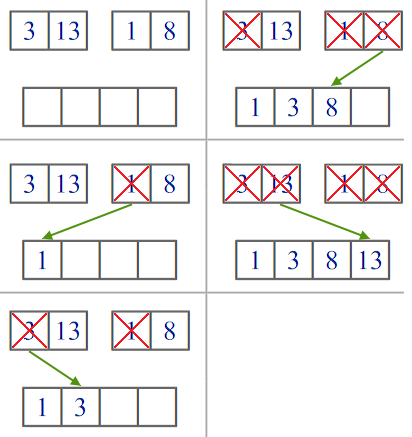
\includegraphics[scale=0.5]{mergesort_example}}
	\caption{Пример работы алгоритма сортировки слиянием}
	\label{figure:image}
\end{figure}

\section{Многопоточность}

\hspace{0.6cm} \textbf {Поток выполнения} — наименьшая единица обработки, исполнение которой может быть назначено ядром операционной системы. Реализация потоков выполнения и процессов в разных операционных системах отличается друг от друга, но в большинстве случаев поток выполнения находится внутри процесса. Несколько потоков выполнения могут существовать в рамках одного и того же процесса и совместно использовать ресурсы, такие как память, тогда как процессы не разделяют этих ресурсов. В частности, потоки выполнения разделяют инструкции процесса (его код) и его контекст (значения переменных, которые они имеют в любой момент времени).

На одном процессоре многопоточность обычно происходит путём временного мультиплексирования (как и в случае многозадачности): процессор переключается между разными потоками выполнения. Это переключение контекста обычно происходит достаточно часто, чтобы пользователь воспринимал выполнение потоков или задач как одновременное. В многопроцессорных и многоядерных системах потоки или задачи могут реально выполняться одновременно, при этом каждый процессор или ядро обрабатывает отдельный поток или задачу.

Потоки возникли в операционных системах как средство распараллеливания вычислений.

Параллельное выполнение нескольких работ в рамках одного интерактивного приложения повышает эффективность работы пользователя. Так, при работе с текстовым редактором желательно иметь возможность совмещать набор нового текста с такими продолжительными по времени операциями, как переформатирование значительной части текста, печать документа или его сохранение на локальном или удаленном диске. Еще одним примером необходимости распараллеливания является сетевой сервер баз данных. В этом случае параллелизм желателен как для обслуживания различных запросов к базе данных, так и для более быстрого выполнения отдельного запроса за счет одновременного просмотра различных записей базы. Именно для этих целей современные ОС предлагают механизм многопоточной обработки (multithreading). Понятию «поток» соответствует последовательный переход процессора от одной команды программы к другой. ОС распределяет процессорное время между потоками. Процессу ОС назначает адресное пространство и набор ресурсов, которые совместно используются всеми его потоками. 

Создание потоков требует от ОС меньших накладных расходов, чем процессов. В отличие от процессов, которые принадлежат разным, вообще говоря, конкурирующим приложениям, все потоки одного процесса всегда принадлежат одному приложению, поэтому ОС изолирует потоки в гораздо меньшей степени, нежели процессы в традиционной мультипрограммной системе. Все потоки одного процесса используют общие файлы, таймеры, устройства, одну и ту же область оперативной памяти, одно и то же адресное пространство. Это означает, что они разделяют одни и те же глобальные переменные. Поскольку каждый поток может иметь доступ к любому виртуальному адресу процесса, один поток может использовать стек другого потока. Между потоками одного процесса нет полной защиты, потому что, во-первых, это невозможно, а во-вторых, не нужно. Чтобы организовать взаимодействие и обмен данными, потокам вовсе не требуется обращаться к ОС, им достаточно использовать общую память — один поток записывает данные, а другой читает их. С другой стороны, потоки разных процессов по-прежнему хорошо защищены друг от друга.

Широко используемый подход состоит и в применении тех или иных библиотек, обеспечивающих определенный программный интерфейс (application programming interface, API) для разработки параллельных программ. В рамках такого подхода наиболее известны Windows Thread API. Однако первый способ применим только для ОС семейства Microsoft Windows, а второй вариант API является достаточно трудоемким для использования и имеет низкоуровневый характер \cite{Barkalov}.

\section{Вывод}

К программе будут применены следующие требования к программному обеспечению.

\vspace{\baselineskip}

\textbf{Требования к вводу:} на вход подаются массив, заполненный случайными числами, индексы первого и последнего элементов. 

\vspace{\baselineskip}

\textbf{Требования к программе:}

\begin{enumerate}
	\item на выходе
	необходимо получить массив, отсортированный по возрастанию;
	\item требуется замерить время работы
	каждого из алгоритмов. 
\end{enumerate}


\chapter{Конструкторская часть}
В этом разделе содержатся cхемы алгоритма сортировки массива слиянием и описание его паралелльной версии.

На вход алгоритм принимает массив, индексы первого и последнего элементов. 
	
\section{Схемы алгоритмов}
На Рис. 2.1 представлена схема алгоритма сортировки массива слиянием.

\vspace{\baselineskip}

\begin{figure}[h]
	\center{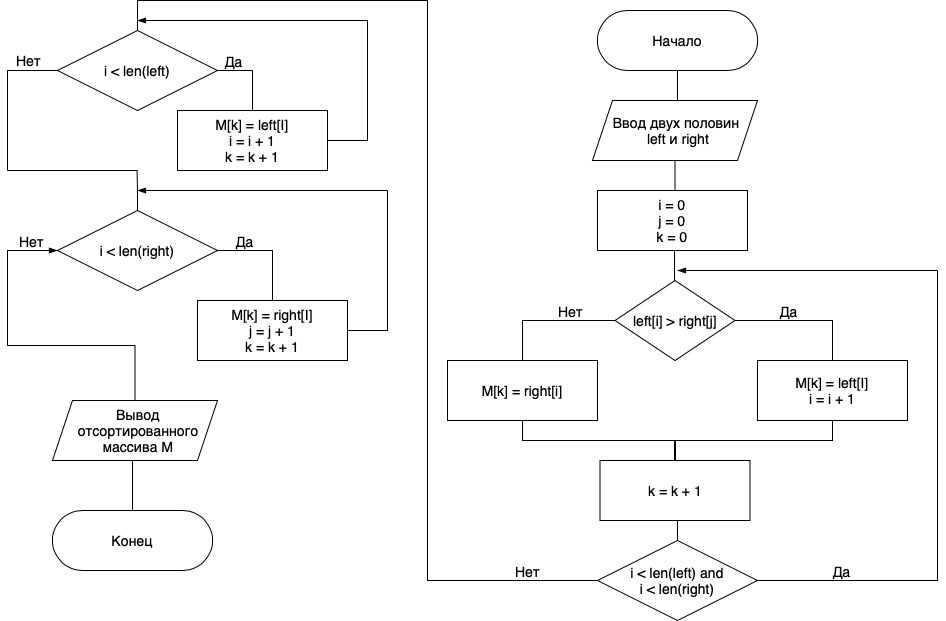
\includegraphics[scale=0.5]{mergesort_bloc}}
	\caption{Схема алгоритма сортировки массива слиянием.}
	\label{figure:image}
\end{figure}

\section{Распараллеливание алгоритма сортировки слиянием}
Распараллеливание программы должно ускорять время работы. Это достигается за счет реализации в узких участках (например, в циклах с большим количеством независимых вычислений).

В предложенном алгоритме данными участком является разделения массива на два подмассива. Данный участок программы как раз предлагается распараллелить.

\chapter{Технологическая часть}
В данном разделе будут рассмотрены требования к программному обеспечению, средства реализации, представлен листинг кода и описание тестирования.

\section{Средства реализации}
В качестве языка программирования был выбран С++ т.к. я знакома с данным языком, у него есть уникальный баланс между возможностями объектно-ориентированного программирования и производительностью. Он одновременно позволяет писать высокоуровневый абстрактный код, который при этом работает со скоростью близкой к машинному коду.

Среда разработки — CLion, которая предоставляет умную проверку кода, быстрое выявление ошибок и оперативное исправление, вкупе с автоматическим рефакторингом кода, и богатыми возможностями в навигации.  

Время работы алгоритмов было замерено с помощью функции steady\_clock() из библиотеки chrono \cite{chrono}. 

Для тестирования использовался компьютер на базе процессора 2,2 GHz Intel Core i7, 6 ядер, 4 логических процессора

Многопоточное программирование было
реализовано с помощью библиотеки pthread \cite{thread}.

\newpage
\section{Листинг кода}

В Листинге 3.1 показана реализация вспомогательной функции для алгоритма сортировки слиянием. Подпрограмма образовывает упорядоченный результирующего массив путем слияния двух также отсортированных массивов меньших размеров.

\begin{flushleft}
Листинг 3.1. Вспомогательной функция для алгоритма сортировки слиянием
\begin{lstlisting}
void merge(int first, int last)
{
	int *mas = new int[M];
	
	int middle = (first + last) / 2;
	int start = first;
	int final = middle + 1;
	
	int j;
	for(j = first; j <= last; j++)
	{
		if ((start <= middle) && ((final > last) || (a[start] < a[final])))
		{
			mas[j] = a[start];
			start++;
		}
		else
		{
			mas[j] = a[final];
			final++;
		}
	}
	for (j = first; j <= last; j++) a[j] = mas[j];
	delete []mas;
}
\end{lstlisting}
\end{flushleft}

\vspace{\baselineskip}

В Листинге 3.2 показана реализация алгоритма сортировки массива слиянием.

\begin{flushleft}
Листинг 3.2. Алгоритм сортировки массива слиянмием
\begin{lstlisting}
int mergesort(void *a, int first, int last)
{
	if (first < last)
	{
		mergesort(a, first, (first+last) / 2);
		mergesort(a, (first+last) / 2 + 1, last);
		
		merge(first, last);
	}
}
\end{lstlisting}
\end{flushleft}

В Листинге 3.3 описана структура для индекса массива
.
\begin{flushleft}
Листинг 3.3. Структура для индекса массива
\begin{lstlisting}
typedef struct Arr {
	int low;
	int high;
} ArrayIndex;
\end{lstlisting}
\end{flushleft}

\vspace{\baselineskip}
	
В Листинге 3.4 показана реализация распараллеленного алгоритма сортировки массива слиянием.

\begin{flushleft}
	Листинг 3.4. Многопоточный алгоритм сортировки массива слиянмием
\begin{lstlisting}
void * mergesort_threads(void *a)
{
	ArrayIndex *pa = (ArrayIndex *)a;
	int mid = (pa->low + pa->high)/2;
	
	ArrayIndex aIndex[N];
	pthread_t thread[N];
	
	aIndex[0].low = pa->low;
	aIndex[0].high = mid;
	
	aIndex[1].low = mid+1;
	aIndex[1].high = pa->high;
	
	if (pa->low >= pa->high) return 0;
	
	int i;
	for(i = 0; i < N; i++) pthread_create(&thread[i], NULL, mergesort_threads, &aIndex[i]);
	for(i = 0; i < N; i++) pthread_join(thread[i], NULL);
	
	merge(pa->low, pa->high);
	
	return 0;
}
\end{lstlisting}
\end{flushleft}

\newpage
\section{Тестирование}
Реализовано функциональное тестирование отдельным файлом test.сpp. Полученные результаты функций сравниваются с контрольными значениями. \vspace{\baselineskip}

Тестирование происходит по следующим данным:
\begin{enumerate}
	\item проверка работы сортировки на массиве размером 1;
	\item проверка работы сортировки на массиве размеров 100, числа расположены случайно;
	\item проверка работы сортировки на массиве размером 100, числа расположеню в порядке убывания;
	\item проверка работы сортировки на массиве размером 100, числа расположеню в порядке возрастания;
\end{enumerate}

Также тестирование проходило сначала стандартым алгоритмом сортировки слиянием, затем его многопоточной версией.

\vspace{\baselineskip}

Программа успешно прошла все тестовые случаи, см. Рис. 3.1. 

\begin{figure}[h]
	\center{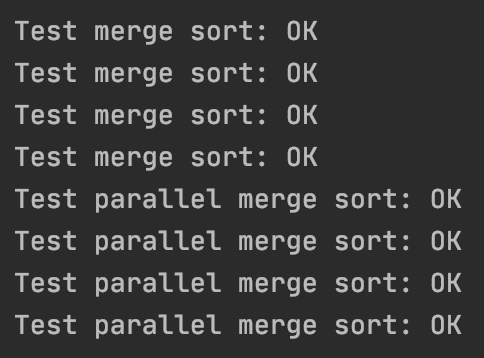
\includegraphics[scale=1]{test_merge}}
	\caption{Тестирование программы}
	\label{figure:image}
\end{figure}

\chapter{Экспериментальная часть}

В данном разделе приведены примеры работы программы и сравнительный анализ алгоритмов на основе экспериментальных данных. 

\section{Примеры работы} 

На Рис. 4.1 приведен пример работы программы.

\begin{figure}[h]
	\center{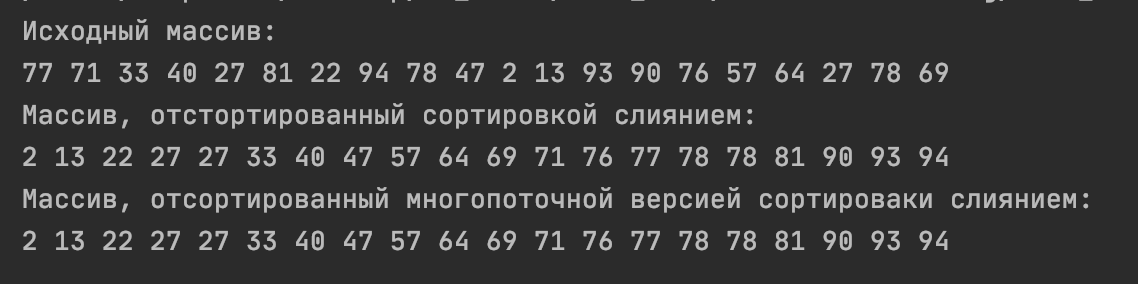
\includegraphics[scale=0.8]{merge_work}}
	\caption{Пример работы программы}
	\label{figure:image}
\end{figure}

\newpage
\section{Постановка эксперимента по замеру времени}

Для произведения замеров времени выполнения реализации алгоритмов будет использована формула: \begin{equation}\label{eq:fourierrow}
	t = \frac{T}{N}
\end{equation}
где t — среднее время выполнения алгоритма, N — количество замеров, T — время выполнения N замеров.  
Неоднократное измерение времени необходимо для получения более точного результа.  
 
Все эксперименты производятся на массивах размеров от 100 до 1000 c шагом 100. Время измеряется в микросекундах.
 
 На рисунке 4.1 изображены графики зависимости времени выполнения программы от размера входных квадратных матриц и количество потоков:  
 
 \begin{center}
 \begin{tikzpicture}
 	\begin{axis}[
 		axis lines = left,
 		xlabel = {Размер матрицы},
 		ylabel = {Время (мкс)},
 		legend pos=north west,
 		ymajorgrids=true
 		]
 		\addplot[color=red, mark=square] table[x index=0, y index= 1] {row_blocks1.txt}; 
 		\addplot[color=green, mark=square] table[x index=0, y index= 1] {row_blocks2.txt}; 
 		\addplot[color=blue, mark=square] table[x index=0, y index= 1] {row_blocks4.txt}; 
 		\addplot[color=orange, mark=triangle] table[x index=0, y index= 1] {row_blocks8.txt}; 
 		\addplot[color=brown, mark=circle] table[x index=0, y index= 1] {row_blocks16.txt}; 
 		
 		\addlegendentry{1 поток}
 		\addlegendentry{2 потока}
 		\addlegendentry{4 потока}
 		\addlegendentry{8 потоков}
 		\addlegendentry{16 потоков}
 		
 	\end{axis}
 \end{tikzpicture}

 	Pис. 4.1: Сравнение времени работы алгоритма работы сортировки слиянием при различном количестве потоков.
 \end{center}
 
Как видно из Рис. 4.3, начиная с 4 потоков увеличение числа потоков не дало сильного прироста в скорости, это связано с тем, что число потоков, которые  работают параллельно равно числу логических процессоров, которых на экспериментальном процессоре, как было сказано в Технологической части, 4.
 
 
 \section*{Вывод}
 \qquad По результатам исследования получилось, что, учитывая количество логических процессоров, программа, работающая на 4-ех потоках, выигрывает по скорости работы по сравнению с программой, которая работает на 1-ом или 2-ух потоках. Исползовать больше потоков, чем логических процессоров на компьютере, неэффективно.
 
\newpage
\chapter*{Заключение}
\addcontentsline{toc}{section}{Заключение}
\hspace{0.6cm}В ходе лабораторной работы были изучены возможности параллельных вычислений и использованы на практике. Был реализован алгоритм сортировки массива слиянием с помощью параллельных вычислений.
Было произведено сравнение работы многотопоточного алгоритма на разном количестве потоков. Эксперементально было установлено, что увеличение потоков имеет смысл, пока не будет достигнуто число логических процессоров в системе, причем максимальная скорость работы достигается именно при нем.
 
 Цель работы достигнута. Получены практические навыки использования параллельных вычислений, а также проведена исследовательская работа по временной эффективности такого подхода.     


\begin{thebibliography}{2}
	\addcontentsline{toc}{chapter}{Список литературы}
	\bibitem{academy} Основные виды сортировок и примеры их реализации. [электронный ресурс]. Режим доступа: https://academy.yandex.ru/posts/osnovnye-vidy-sortirovok-i-primery-ikh-realizatsii
	(Дата обращения: 16.10.2020)
	\bibitem{Barkalov}
	Константин Баркалов, Владимир Воеводин, Виктор Гергель. Intel Parallel Programming [электронный ресурс]. Режим доступа: https://www.intuit.ru/studies/courses/4447/983/lecture/14925, свободный (Дата обращения: 15.10.20)
	\bibitem{voevodin}Воеводин В. В., Воеводин Вл. В. Параллельные вычисления. — СПб: БХВ-Петербург, 2002. — 608 с.
	\bibitem{chrono} Официальный сайт Microsoft, документация [электронный ресурс]. Режим доступа: https://docs.microsoft.com/ru-ru/cpp/standard-library/chrono?view=vs-2017, свободный (Дата обращения: 15.10.20)
	\bibitem{thread} Официальный сайт Microsoft, документация [электронный ресурс]. Режим доступа: https://docs.microsoft.com/ru-ru/cpp/standard-library/thread-class?view=vs-2019, свободный (Дата обращения: 15.10.20)
	
\end{thebibliography}
\end{document}